\documentclass[a4paper,11pt]{article}
\usepackage[utf8]{inputenc}
\usepackage{algorithmic}
\usepackage{algorithm}
\usepackage{pst-plot}
\usepackage{graphicx}
\usepackage{endnotes}
\usepackage{graphics}
\usepackage{floatflt}
\usepackage{wrapfig}
\usepackage{amsfonts}
\usepackage{amsmath}
\usepackage{verbatim}
\usepackage{hyperref}
\usepackage{multirow}
\usepackage{pdflscape}
 \usepackage{enumitem}

\usepackage{hyperref}
\hypersetup{pdfborder={0 0 0 0}}

\pdfpagewidth 210mm
\pdfpageheight 297mm 
\setlength\topmargin{0mm}
\setlength\headheight{0mm}
\setlength\headsep{0mm}
\setlength\textheight{250mm}	
\setlength\textwidth{159.2mm}
\setlength\oddsidemargin{0mm}
\setlength\evensidemargin{0mm}
\setlength\parindent{7mm}
\setlength\parskip{0mm}

\newenvironment{exercise}[3]{\paragraph{Exercise #1: #2 (#3pt)}\ \\}{
\medskip}
\newcommand{\question}[2]{\setlength\parindent{0mm}\ \\$\mathbf{Q_{#1}:}$ #2\ \\}

\author{\large{Ilya Kuzovkin, Raul Vicente}}
\title{\huge{Introduction to Computational Neuroscience}\\\LARGE{Practice VIII: Brain-Computer Interfaces}}

\begin{document}
\maketitle


%
% Intro
%
\ \\
Brain-Computer Interface (BCI) is a common name for all kinds of systems that use brain signals to control external devices (cursors, computers, wheelchairs, robots, etc.). All kinds of neuroimaging techniques are used to create BCIs. Each technique has it's own advantages and disadvantages. BCIs are divided into two large groups: invasive and non-invasive. The former ones provide much better accuracy, but require surgery and therefore are not applicable to every user. The non-invasives on the other hand provide much lesser spatial and/or temporal resolutions, resulting in much worse performance of a BCI system. Provided that an average person will not allow to implant electrodes in his brain in near future the non-invasive techniques are worth exploring nevertheless.

\ \\
\textbf{Request:} Please record the time you will spend of this homework and add it to the report. This is just for me to balance the amount and the difficulty level of the exercises.

%
% Questionnaire
%
\begin{exercise}{1}{Questionnaire}{0.5}
\question{1}{Explain how machine learning is used in BCI. What is taken as a training set, what plays a role of a test set, what are the classes, what are the features.}
\question{2}{What are advantages and disadvantages of microelectrode-based BCIs?}
\question{3}{What are advantages and disadvantages of EEG-based BCIs?}
\question{4}{What are advantages and disadvantages of fMRI-based BCIs?}
\question{5}{Which BCI technique relies on the fact that if the test subject is looking at the stimulus flashing with frequency $f$ then in the recorded brain signal the power of the periodic component with the frequency $f$ rises?}
\end{exercise}


%
% 
%
\begin{exercise}{2}{Invasive: ECoG data}{2 + 1* }
In this exercise we will use the data recorded using an ECoG\footnote{\url{http://en.wikipedia.org/wiki/Electrocorticography}} array. The data was recorded from three test subject, while they were flexing their fingers (see Figure \ref{fig:fingers})
\begin{figure}[H]
   \centering
   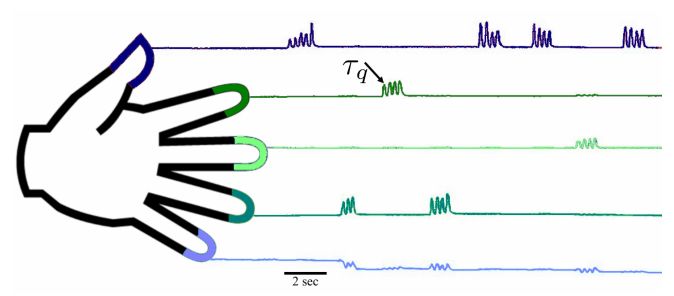
\includegraphics[width=0.7\textwidth]{fingers.png} 
   \caption{We want to identify finger flexion from ECoG data.}
   \label{fig:fingers}
\end{figure}
\ \\
The underlying BCI application for this data is the task of predicting flexion of the fingers from the brain data. You can imagine that this can be used to control a finger flexion of a robotic hand. This dataset and the task of predicting the finger flexions was proposed as a part of the BCI Competition IV\footnote{\url{http://bbci.de/competition/iv}}. The success of the predictive model is measured using correlation between the two time series: the true finger flexion and the predicted flexion. On Figure \ref{fig:predicted} you can see an example. Run the code in the \texttt{exercise2.m} to see how it is achieved.
\begin{figure}[H]
   \centering
   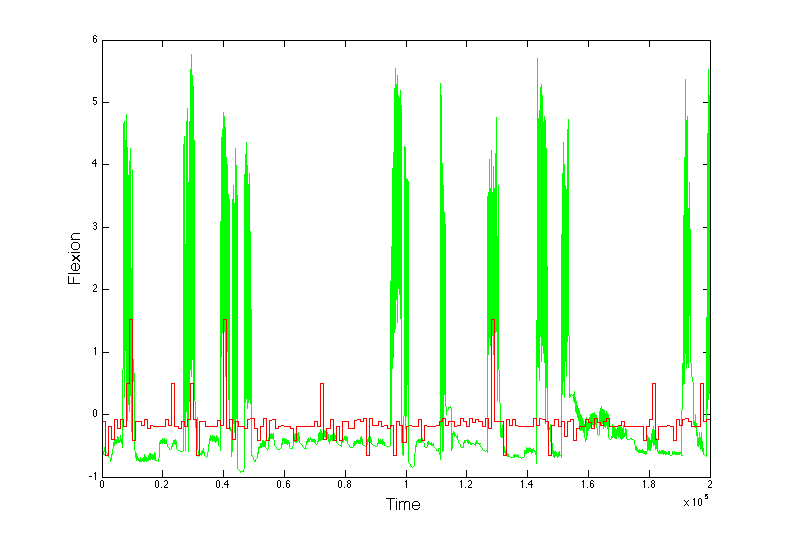
\includegraphics[width=0.7\textwidth]{predicted.png} 
   \caption{The green line shows the true flexions of the finger \#1 (thumb) of the test subject \#1, the red one is the predicted flexions. The correlation between these two time series is 0.2374.}
   \label{fig:predicted}
\end{figure}

\ \\
In this exercise you will have to do the following:
\begin{itemize}
\itemsep 0em
	\item Read the data and competition description here: \url{http://bbci.de/competition/iv/desc_4.pdf}
	\item Plot one second of the ECoG data from one channel. Report the figure. This is just to see how the data looks like.
	\item Plot the thumb (1st finger) flexion over the whole period of training (400 seconds).
	\item See how the correlation for finger 1 is computed.
	\item Compute the correlations for fingers 2, 3, 5 (4th finger is omitted). Report the correlations and the figures.
	\item Compute the average correlation for this test subject. Report it.
	\item Compute the average correlations for other two test subjects. Report them.
	\item Compute the average correlation over all three subjects. Report it.
	\item Compare the result you got with the results of the competition: \url{http://bbci.de/competition/iv/results/index.html#dataset4}
\end{itemize}
By now you have earned 1.5 points. Let's move on:
\begin{itemize}
\itemsep 0em
	\item Try to change the parameters of the system to achieve better results:
	\begin{itemize}
		\item Window size
		\item Features
	\end{itemize}
	\item Report what you did and how it affected the final score (overall average correlation)
\end{itemize}
\ \\
Now you have 2 points, but you can squeeze additional bonus point from this exercise:
\begin{itemize}
	\item Try to achieve even better result (higher overall correlation value) by trying whatever comes to your mind:
	\begin{itemize}
		\item Floating window
		\item Specific sets of features
		\item Different machine learning algorithms
		\item ...
	\end{itemize}
	\item Send the correlation value you achieved and short description of how you did it to the course mailing list (\url{aine.ati.neuro@lists.ut.ee}). If your correlation is higher than the one you got in the first part of the exercise (default code) and it is higher than the previous submitted result then you get \textbf{1 bonus point}.
\end{itemize}

\paragraph{Note 1:} Let me remind you that the final score (total average correlation) is computed as
$$c = \displaystyle\frac{\displaystyle\frac{C^1_1 + C^1_2 + C^1_3 + C^1_5}{4} + \frac{C^2_1 + C^2_2 + C^2_3 + C^2_5}{4} + \frac{C^3_1 + C^3_2 + C^3_3 + C^3_5}{4}}{3}$$
where $C^s_f$ for subject $s$ and finger $f$ is computed as
$$C^s_f = \mathbf{corr}(\text{true flexions of finger $f$ of subject $s$}, \text{predicted flexions of finger $f$ of subject $s$})$$
Notice that finger 4 is omitted from the equation.

\paragraph{Note 2:} You are not allowed to create models which are specific to the test subjects. So the solution which uses one model for one subject and another model for another subject does not count.

\end{exercise}


%
% Discuss
%
\begin{exercise}{3}{Examples of BCIs}{0.5}
Use your favorite source of information to find some example of BCI systems, good places to start from are:
\begin{itemize}
\itemsep 0em
	\item Google Scholar: \url{http://scholar.google.com/scholar?hl=en&q=brain+computer+interface}
	\item Youtube: \url{https://www.youtube.com/results?search_query=brain+computer+interface}
	\item Plain Google: \url{https://www.google.com/search?q=brain-computer+interface}
\end{itemize}
Present the following information:
\begin{itemize}
\itemsep 0em
	\item Video or a picture
	\item What neuroimaging technology do they use?
	\item Name and year of the article.
	\item What is the task of this BCI system? How many classes/actions?
	\item How accurate the system is?
	\item Which machine learning (or other) method do they use?
\end{itemize}
\end{exercise}


\ \\
\ \\
\ \\
\ \\
\ \\
Please submit a PDF report with answers to the questions and comments about your solutions. You report should contain figures, explanations, the essential parts of the code you have produced, etc. If the code is too massive you can add it to the submission and upload everything as a \texttt{zip} archive. But single PDF is preferred.

\end{document}










